\documentclass[
  sigplan,
  10pt,
  %anonymous,
  %review,
  ]{acmart}
\settopmatter{printfolios=true,printccs=false,printacmref=false}

\usepackage[british]{babel}

\usepackage{mathpartir}

%\usepackage{unicode-math}
%\setmathfont{latinmodern-math.otf}
%\setmathfont[version=bold, FakeBold=2]{latinmodern-math.otf}

% Record brackets
\usepackage{stmaryrd}

\usepackage{xcolor}

\usepackage{tikz}
\usepackage{pgfplots}

\usepackage{enumitem}

\usepackage{array}
\usepackage{multirow}

\usepackage{listings}
\definecolor{isarblue}{HTML}{006699}
\definecolor{isargreen}{HTML}{009966}
\lstdefinelanguage{isabelle}{%
    keywords=[1]{type_synonym,datatype,fun,function,abbreviation,definition,proof,lemma,theorem,corollary,inductive},
    keywordstyle=[1]\bfseries\color{isarblue},
    keywords=[2]{where,assumes,shows,and,fixes},
    keywordstyle=[2]\bfseries\color{isargreen},
    keywords=[3]{if,then,else,case,of,SOME,let,in,O},
    keywordstyle=[3]\color{isarblue},
}
\lstset{%
  language=isabelle,
  escapeinside={&}{&},
  columns=\lst@ifdisplaystyle{fullflexible}\else{fixed}\fi,,
  extendedchars,
  basewidth={0.5em,0.45em},
  basicstyle=\ttfamily,
  mathescape,
}
\makeatletter
\lst@AddToHook{OnEmptyLine}{\vspace{-0.4\baselineskip}}
\makeatother
\newcommand{\lstinlinew}[2][]{\lstinline[#1]{#2}}
% This is a hack to allow escaping inside lstinline (https://tex.stackexchange.com/questions/43526/escaping-in-lstinline)
\usepackage{etoolbox}
\makeatletter
\patchcmd{\lsthk@TextStyle}{\let\lst@DefEsc\@empty}{}{}{\errmessage{failed to patch}}
\makeatother

\usepackage{calc}

\newcommand{\textover}[3][l]{%
 % #1 is the alignment, default l
 % #2 is the text to be printed
 % #3 is the text for setting the width
 \makebox[\widthof{#3}][#1]{#2}%
}

\hyphenation{Isa-belle}
\hyphenation{tab-leau}

% For arXiv: LuaLatex on Arxiv: https://tex.stackexchange.com/questions/372154/lualatex-how-to-produce-pdf-acceptable-by-arxiv 
%\hypersetup{%
%  pdfcreator = {},
%  pdfproducer = {}
%}
%\pdfvariable suppressoptionalinfo \numexpr 1+2+4+8+16+32+64+128+256+512 \relax

% For arXiv: Remove copyright information
% \setcopyright{none}
% \renewcommand\footnotetextcopyrightpermission[1]{}


\usepackage{todonotes}

% Autoref names
\renewcommand{\sectionautorefname}{Section}
\renewcommand{\subsectionautorefname}{Section}

% Commands
\newcommand{\MLSS}{\textbf{MLSS}}

\newlength{\trianglewidth}
\settowidth{\trianglewidth}{\(\triangleleft\)}
\newcommand{\lefttrianglebar}{\mathrel{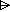
\includegraphics{./symbols/lefttrianglebar.pdf}}}
\newcommand{\lefttriangle}{\mathrel{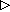
\includegraphics{./symbols/lefttriangle.pdf}}}

\newcommand{\lexpands}[2]{#1 $\lefttriangle$ #2}
\newcommand{\fexpands}[2]{#1 $\lefttrianglebar$ #2}
\newcommand{\fexpandsW}[2]{#1 $\lefttrianglebar_\text{v}$ #2}
\newcommand{\expandssSym}{\lefttriangle^*}
\newcommand{\expandss}[2]{#1 $\expandssSym$ #2}

\newcommand{\unionS}{\sqcup_\text{s}}
\newcommand{\interS}{\sqcap_\text{s}}
\newcommand{\diffS}{-_\text{s}}
\newcommand{\inS}{\in_\text{s}}
\newcommand{\notinS}{\notin_\text{s}}
\newcommand{\eqS}{=_\text{s}}
\newcommand{\neqS}{\neq_\text{s}}
\newcommand{\subseteqS}{\sqsubseteq_\text{s}}
\newcommand{\Ist}{I$_\text{st}$}
\newcommand{\Isa}{I$_\text{sa}$}

\newcommand{\fmAnd}[2]{#1 $\boldsymbol{\land}$ #2}
\newcommand{\fmOr}[2]{#1 $\boldsymbol{\lor}$ #2}
\newcommand{\fmNegSymbol}{\boldsymbol{\neg}}
\newcommand{\fmNeg}[1]{$\fmNegSymbol$ #1}
\newcommand{\fmAtom}{\textbf{A}}

\begin{document}

% For arXiv: Remove conference/author in the header
% \pagestyle{plain}

\setcounter{tocdepth}{1}

\title{Towards a Verified Tableau Prover for a Ground Fragment of Set Theory}
\author{Lukas Stevens}
\orcid{0000-0003-0222-6858}
\affiliation{%
  \institution{Technical University of Munich}
  \department{Department of Informatics}
  \streetaddress{Boltzmannstr. 3}
  \city{Garching}
  \postcode{85748}
  \country{Germany}
}
\email{lukas.stevens@in.tum.de}

\begin{abstract}
  Using Isabelle/HOL, we verify the state-of-the-art decision procedure for multi-level syllogistic with singleton (\MLSS{} for short), which is a ground fragment of set theory.
  We formalise the syntax and semantics of \MLSS{} as well as a sound and complete tableau calculus for it.
  We also provide an abstract specification of a decision procedure that applies the rules of the calculus exhaustively and prove its termination.
\end{abstract}

\maketitle

\listoftodos{}

\section{Introduction}
In contrast to pen-and-paper proofs where we expect the reader to fill in trivial details, interactive theorem provers (ITPs) require us to justify each proof step rigorously.
\todo[inline]{Reviewer: Reformulate below because we can use cuts}
Manually reducing each proof step down to the axioms would be impractical, though;
hence, ITPs usually offer a wide array of automated methods to deal with the proof goals that arise during interactive use.

In Isabelle/HOL, there are specialised procedures for dealing with e.g.\ natural numbers, linear arithmetic, and metric spaces.
Some of these procedures have been verified in Isabelle/HOL such as a procedure for Presburger arithmetic~\cite{presburger} that was later extended to mixed real-integer arithmetic~\cite{arithmetic}.
This procedure, though, uses reflection to work on goals in Isabelle/HOL, which, during execution, either sacrifices speed by going through the simplifier or soundness by trusting generated code.
More recently, \citeauthor{orders}~\cite{orders} presented a verified decision procedure for orders that produces certificates. 
This approach offers efficient execution by using generated code as well as soundness as the certificates are replayed through Isabelle's inference kernel.

The focus of this paper is another ubiquitous structure in mathematics, namely sets.
In particular, we consider a ground fragment of set theory which \citeauthor{new_fast_tableau}~\cite{new_fast_tableau} call multi-level syllogistic with singleton (\MLSS{}).
The fragment includes the usual set operations of union, intersection, difference, membership, equality and, in addition, it allows the construction of singleton sets.
Due to the omnipresence of sets, we think that automation for this fragment will benefit the users of Isabelle, especially when integrated into the simplifier like the aforementioned order solver.
We also expect that the generation of certificates will be straightforward since \MLSS{} admits a tableau calculus.

\subsection{Contributions}
In this paper, we present a formalisation in Isabelle/HOL of a tableau calculus for \MLSS{} due to \citeauthor{new_fast_tableau}~\cite{new_fast_tableau}\cite[Chapter 14]{set_theory}.
We prove soundness and completeness of the calculus and give an abstract specification of a decision procedure that applies the rules of the calculus exhaustively.
To obtain total correctness of the procedure, we prove its termination.
The formalisation follows the paper closely but gives a more thorough account of some important details:
\begin{itemize}
  \item We deliver the omitted proof of Lemma~2 in the paper~\cite{new_fast_tableau}, which is a key building block for the completeness proof of the calculus.
  \item The formal proof of completeness lead to the discovery that the calculus was missing a rule for eliminating double negation. 
  \item We derive an explicit upper bound for the number of formulae in a branch of the tableau.
\end{itemize}

\subsection{Related Work}
Since the literature on decidable fragments of set theory is vast, we only focus on \MLSS{} here.
The fragment was first shown to be decidable by \citeauthor{mlss_first}~\cite{mlss_first}.
Subsequent work~\cite{mlss_np} found the decision problem to be \textbf{NP}-complete.
To obtain a practical decision procedure, \citeauthor{mlss_first_tableau}~\cite{mlss_first_tableau} proposed a tableau calculus, which was later improved by \citeauthor{tableau_quantifier_free}~\cite{tableau_quantifier_free}.
Both of these procedures construct a model during execution that is used to guide the proof search.
\citeauthor{tableau_quantifier_free} also cover an extension of the calculus with uninterpreted functions, which was revisited by \citeauthor{mlss_quantification}~\cite{mlss_quantification} who avoided the construction of a model during execution.
In this paper, we consider a version of the latter procedure due to \citeauthor{new_fast_tableau}~\cite{new_fast_tableau} that is specialised to \MLSS{} and where the branching rules of the calculus are set up in a way to guarantee mutual exclusivity of the branches.
Later extensions of the calculus added certain interpreted functions such as monotone functions~\cite{mlss_monotone_functions} and the inverse of a function~\cite{mlss_cartesian_map}.
The latter extension notably includes the Cartesian product.
Those extensions, though, did not improve upon the tableau calculus for \MLSS{}.

While a lot of work has gone into the verification of decision procedures, seemingly little has been put towards the verification of tableau calculi.
In Lean, there is a verified tableau calculus for basic modal logic~\cite{modal_logic_lean}.
In Coq, there is a formalisation of a tableau calculus for ecumenical logic~\cite{ecumenical_logic}; it is, however, missing a completeness proof.
Concerning Isabelle/HOL, there is formalisation of a sound and complete tableau calculus for hybrid logic~\cite{hybrid_logic} available in the \textit{Archive of Formal Proofs}~\cite{hybrid_logic_afp}.
The termination proof is part of ongoing work~\cite{hybrid_logic_workshop}.
% TODO: Formalisation de la logique temporelle dans le coq.

\subsection{Notation}
Isabelle/HOL~\cite{isabelle} conforms to everyday mathematical notation for the most part.
We establish notation and in particular some essential data types together with their primitive operations that are specific to Isabelle/HOL.

We write \lstinline!t :: 'a! to specify that the term \lstinline!t! has the type \lstinline!'a! and \lstinline!'a $\Rightarrow$ 'b! for the space of total functions from type \lstinline!'a! to type \lstinline!'b!.

Sets with elements of type \lstinline!'a! have the type \lstinline!'a set!.
The cardinality of a set \lstinline!A! is denoted by \lstinline!card A! and the image of \lstinline!A! under \lstinline!f! by \lstinline!f ` A!.

We use \lstinline!'a list! to describe the type of lists, which are constructed using the empty list \lstinline![]! constructor or the infix cons constructor \lstinline!#!, and are appended with the infix operator \lstinline!@!.
The function \lstinline!set! converts a list into a set.

We remark that $\longleftrightarrow$ is equivalent to \lstinline!$=$! on the type of Booleans \lstinline!bool! and \lstinline!$\equiv$! is definitional equality of the meta-logic of Isabelle/HOL, which is called Isabelle/Pure.
Meta-implication is denoted by \lstinline!$\Longrightarrow$! and a chain of implications
\begin{lstlisting}
  A$_\text{1}$ $\Longrightarrow$ $\cdots$ $\Longrightarrow$ A$_\text{k}$ $\Longrightarrow$ C
\end{lstlisting}
can be abbreviated by 
\begin{lstlisting}
  $\llbracket$ A$_\text{1}$;$\,\ldots\,$;A$_\text{k}$ $\rrbracket$ $\Longrightarrow$ C.
\end{lstlisting}

\section{Syntax and Semantics of MLSS\label{sec:semantics}}
\subsection{Syntax}
At the heart of \MLSS{}, we have the type of set terms which is the disjoint union of the empty set and variables as well as the operations union, intersection, set difference, and the singleton set represented by the constructor \lstinline!Single!.
We keep the type of variables abstract by making it a parameter of the set term data type.
The only restriction on the type of variables is that it needs to be infinite.
Isabelle/HOL's data type package automatically defines a function that gives us the set of variables in a set term, which we name \lstinline!vars!.
In what follows, we will overload the function \lstinline!vars! to also work on set atoms, formulae, and branches.
\begin{lstlisting}
datatype (vars: 'a) pset_term =
  $\emptyset$ | Var 'a | Single ('a pset_term)
| 'a pset_term $\unionS$ 'a pset_term
| 'a pset_term $\interS$ 'a pset_term
| 'a pset_term $\diffS$ 'a pset_term
\end{lstlisting}
We can combine two set terms to form a set atom by using the membership or the equality operator.
\begin{lstlisting}
datatype (vars: 'a) pset_atom =
  'a pset_term $\inS$ 'a pset_term
| 'a pset_term $\eqS$ 'a pset_term
\end{lstlisting}
With the above operators we can also represent the subset operator \lstinline!$\subseteqS$! and enumerate finite sets: \lstinline!s $\subseteqS$ t! is equivalent to \lstinline!s $\unionS$ t $\eqS$ t! and a finite set of elements \lstinline!{t$_\text{1}$,$\ldots$,t$_\text{k}$}! can be expressed by \lstinline!Single t$_1$ $\unionS$ $\ldots$ $\unionS$ Single t$_k$!.

We use the propositional fragment of formulae due to \citeauthor{lqe}~\cite{lqe} with set atoms as propositional atoms to form the unquantified fragment \MLSS{} of set theory.
\begin{lstlisting}
datatype (atoms: 'a) fm =
  &\fmAtom& 'a | &\fmNeg{('a fm)}&
| &\fmAnd{'a fm}{'a fm}& | &\fmOr{'a fm}{'a fm}&

type_synonym 'a pset_fm = 'a pset_atom fm
\end{lstlisting}
We will often drop the atom constructor \lstinline!&\fmAtom{}&! to reduce clutter.
Additionally, we use the abbreviations \lstinline!s $\notinS$ t! and \lstinline!s $\neqS$ t! to denote \lstinline!&\fmNeg{\fmAtom{} (s $\inS$ t)}&! and \lstinline!&\fmNeg{\fmAtom{} (s $\eqS$ t)}&!, respectively.

Like the function \lstinline!vars!, the automatically defined function \lstinline!atoms :: 'a fm $\Rightarrow$ 'a set! retrieves all set atoms in a formula.
We combine these functions to extract all the variables occurring in a set formula.
\begin{lstlisting}
definition vars :: 'a pset_fm $\Rightarrow$ 'a set where
  vars $\phi$ $\equiv$ $\bigcup$(vars ` atoms $\phi$)
\end{lstlisting}

Similarly to \lstinline!vars!, we introduce the overloaded constant \lstinline!subterms!.
\begin{lstlisting}
fun subterms :: 'a pset_term
             $\Rightarrow$ 'a pset_term set where
  subterms $\emptyset$ = {$\emptyset$}
| subterms (Var x) = {Var x}
| subterms (s $\unionS$ t) =
    {s $\unionS$ t} $\cup$ subterms s $\cup$ subterms t
| subterms (s $\interS$ t) =
    {s $\interS$ t} $\cup$ subterms s $\cup$ subterms t
| subterms (s $\diffS$ t) =
    {s $\diffS$ t} $\cup$ subterms s $\cup$ subterms t
| subterms (Single t) =
    {Single t} $\cup$ subterms t
\end{lstlisting}
The subterms of an atom are then the subterms of its arguments.
\begin{lstlisting}
fun subterms :: 'a pset_atom
             $\Rightarrow$ 'a pset_term set where
  subterms (s $\inS$ t) = subterms s $\cup$ subterms t
| subterms (s $\eqS$ t) = subterms s $\cup$ subterms t
\end{lstlisting}
Finally, we lift this to formulae by using \lstinline!atoms! again.
\begin{lstlisting}
definition subterms ::
    'a pset_fm $\Rightarrow$ 'a pset_term set where
  subterms $\phi$ $\equiv$ $\bigcup$(subterms ` atoms $\phi$)
\end{lstlisting}

Lastly, we consider the subformulae of a formula and define a function that computes them.
\begin{lstlisting}
fun subfms :: 'a fm $\Rightarrow$ 'a fm set where
  subfms (&\fmAtom& a) = {&\fmAtom& a}
| subfms (&\fmAnd{p}{q}&) =
    {&\fmAnd{p}{q}&} $\cup$ subfms p $\cup$ subfms q
| subfms (&\fmOr{p}{q}&) =
    {&\fmOr{p}{q}&} $\cup$ subfms p $\cup$ subfms q
| subfms (&\fmNeg{q}&) = {&\fmNeg{q}&} $\cup$ subfms q
\end{lstlisting}
\textit{Literals} are a type of subformulae of particular importance, so we define a predicate for them.
\begin{lstlisting}
fun is_literal :: 'a fm $\Rightarrow$ bool where
  is_literal (&\fmAtom& _) = True
| is_literal (&\fmNeg{(\fmAtom{} \_)}&) = True
| is_literal _ = False
\end{lstlisting}
\subsection{Semantics}
We base the semantics of \MLSS{} on the von Neumann hierarchy $\mathcal{V}$ of sets that is defined inductively as
  \[
    \begin{array}{rclr}
      \mathcal{V}_0 & = & \emptyset, \\
      \mathcal{V}_{\alpha + 1} & = & \mathcal{P}(\mathcal{V}_\alpha) & \text{for each ordinal $\alpha$}, \\
      \mathcal{V}_{\lambda} & = & \bigcup_{\mu < \lambda} \mathcal{V}_\mu & \text{for each limit ordinal $\lambda$}, \\
      \mathcal{V} & = & \bigcup_\alpha \mathcal{V}_\alpha, \\
    \end{array}
  \]
where $\mathcal{P}(S)$ is the powerset of $S$.
The sets in $\mathcal{V}$ are well-founded, i.e.\ there can be no membership cycle in $\mathcal{V}$.

In Isabelle/HOL, which is simply typed, this definition is not accepted, though.
A way to work around this limitation is provided by \citeauthor{zfc_in_hol_afp} in an entry~\cite{zfc_in_hol_afp} of the \textit{Archive of Formal Proofs}, which adds $\mathcal{V}$ to Isabelle/HOL by way of axiomatisation.
Two articles~\cite{zfc_in_hol1,zfc_in_hol2} have been written that provide further context to this entry.
The entry declares a type \lstinline!V! that comes with the following functionality:
\begin{itemize}
  \item The function \lstinline!elts :: V $\Rightarrow$ V set! maps a set to its elements.
      Note that even though we use the typed sets provided by Isabelle/HOL here, \lstinline!elts! actually returns a class (relative to \lstinline!V!).
      This class only constitutes a set (relative to \lstinline!V!) if the class is small.
  \item The predicate \lstinline!small :: 'a set $\Rightarrow$ bool!, which is polymorphic in \lstinline!'a!, indicates whether a class is small.
  \item The function \lstinline!vset :: 'a set $\Rightarrow$ V! turns a class into a set of type \lstinline!V! if it is small. 
\item The usual set operations such as equality ($=$), union ($\sqcup$), intersection ($\sqcap$), and difference ($-$) are defined.
\item Finally, the empty set coincides with the ordinal $0$, so it is denoted by \lstinline!0 :: V!.
\end{itemize}

Equipped with the above, we define the interpretation function \lstinline!&\Ist&! for set terms that interprets a set term with respect to a valuation function \lstinline!M :: 'a $\Rightarrow$ V! for variables.
\begin{lstlisting}
fun &\Ist& :: ('a $\Rightarrow$ V) $\Rightarrow$ 'a pset_term $\Rightarrow$ V where
  &\Ist& M $\emptyset$ = 0
| &\Ist& M (Var x) = M x
| &\Ist& M (Single s) = vset {&\Ist& M s}
| &\Ist& M (s $\unionS$ t) = &\Ist& M s $\sqcup$ &\Ist& M t 
| &\Ist& M (s $\interS$ t) = &\Ist& M s $\sqcap$ &\Ist& M t 
| &\Ist& M (s $\diffS$ t) = &\Ist& M s $-$ &\Ist& M t 
\end{lstlisting}
The interpretation function \lstinline!I$_\text{sa}$! for set atoms is straightforward as well.
\begin{lstlisting}
fun &\Isa& :: ('a $\Rightarrow$ V) $\Rightarrow$ 'a pset_atom $\Rightarrow$ bool
where
  &\Isa& M (s $\inS$ t) $\longleftrightarrow$ &\Ist& M s $\in$ elts (&\Ist& M t)
| &\Isa& M (s $\eqS$ t) $\longleftrightarrow$ &\Ist& M s = &\Ist& M t
\end{lstlisting}

We write \lstinline!M $\models$ $\phi$! for the judgement that the formula $\phi$ holds under the valuation function \lstinline!M!.
The implementation of $\models$ coincides with the interpretation function of \citeauthor{lqe}~\cite{lqe}.
As usual, a formula \lstinline!$\phi$! is called \textit{satisfiable} if there exists a model \lstinline!$M$! with \lstinline!$M$ $\models$ $\phi$!.
Otherwise, \lstinline!$\phi$! is called \textit{unsatisfiable}.

\section{A Tableau Calculus for MLSS}
We formalise the tableau calculus for \MLSS{} as described by \citeauthor{new_fast_tableau}~\cite{new_fast_tableau}.
Inspired by the formalisation of a tableau calculus for hybrid logic by \citeauthor{hybrid_logic_afp}~\cite{hybrid_logic_afp}, we simply use a list to represent a branch of the tableau tree.
Note that formulae are added to the front of the list during branch expansion, so \lstinline!last b! for a branch \lstinline!b! is always the formula that we are trying to disprove with the tableau. 
\begin{lstlisting}
type_synonym 'a branch = 'a pset_fm list
\end{lstlisting}
We now lift the functions that extract the variables respectively subterms of formulae to branches.
\begin{lstlisting}
definition vars :: 'a branch $\Rightarrow$ 'a set 
  vars b $\equiv$ $\bigcup$(vars ` set b)

definition subterms ::
    'a branch $\Rightarrow$ 'a pset_term set where
  subterms b $\equiv$ $\bigcup$(subterms ` set b)
\end{lstlisting}
In the standard tableau calculus for propositional logic as \citeauthor{tableau}~\cite{tableau} describes it, a branch is called \textit{closed} if it contains both the negation of a formula and the formula itself;
conversely, it is called \textit{open} if it is not closed.
For \MLSS{}, we extend the notion of closedness with three additional rules; the first two are straightforward while the last one states that a branch is closed when the branch contains a membership cycle
\begin{lstlisting}
  t$_\text{0}$ $\inS$ t$_\text{1}$, t$_\text{1}$ $\inS$ t$_\text{2}$, $\ldots$, t$_\text{k}$ $\inS$ t$_\text{0}$.
\end{lstlisting}

\begin{lstlisting}
inductive bclosed :: 'a branch $\Rightarrow$ bool where
  $\llbracket$ $\phi$ $\in$ set b; &\fmNeg{$\phi$}& $\in$ set b $\rrbracket$ $\Longrightarrow$ bclosed b
| (t $\inS$ $\emptyset$) $\in$ set b $\Longrightarrow$ bclosed b
| (t $\neqS$ t) $\in$ set b $\Longrightarrow$ bclosed b
| $\llbracket$ member_cycle cs; set cs $\subseteq$ set b$\rrbracket$
    $\Longrightarrow$ bclosed b

abbreviation bopen b $\equiv$ $\neg$ bclosed b
\end{lstlisting}
A tableau is called \textit{closed} if all of its branches are closed.

\subsection{Linear Expansion Rules}
\begin{table*}
  \lstset{
    escapeinside={@}{@}
  }
  \newcommand{\ton}{\text{t}_\text{1}}
  \newcommand{\ttw}{\text{t}_\text{2}}
  \begin{tabular}{p{0.21\textwidth}cp{0.18\textwidth} p{0.01\textwidth} p{0.21\textwidth}cp{0.18\textwidth}}
    \toprule
    \multicolumn{3}{c}{Propositional Rules} && \multicolumn{3}{c}{Rules for \lstinline!$\unionS$!} \\
    \cmidrule{1-3}\cmidrule{5-7}
    \lstinline!@\fmAnd{p}{q}@! & $\Longrightarrow$ & \lstinline!p, q! &&
    \lstinline!s $\notinS$ $\ton$ $\unionS$ $\ttw$! & $\Longrightarrow$ & \lstinline!s $\notinS$ $\ton$, s $\notinS$ $\ttw$! \\

    \lstinline!@\fmNeg{(\fmOr{p}{q})}@! & $\Longrightarrow$ & \lstinline!@\fmNeg{p}@, @\fmNeg{q}@! &&
    \lstinline!s $\inS$ $\ton$! & $\Longrightarrow$ & \lstinline!s $\inS$ $\ton$ $\unionS$ $\ttw$! \\

    \lstinline!@\fmOr{p}{q}, \fmNeg{p}@! & $\Longrightarrow$ & \lstinline!q! &&
    \lstinline!s $\in$ $\ttw$! & $\Longrightarrow$ & \lstinline!s $\inS$ $\ton$ $\unionS$ $\ttw$! \\

    \lstinline!@\fmOr{p}{q}, \fmNeg{q}@! & $\Longrightarrow$ & \lstinline!p! &&
    \lstinline!s $\inS$ $\ton$ $\unionS$ $\ttw$, s $\notinS$ $\ton$! & $\Longrightarrow$ & \lstinline!s $\inS$ $\ttw$! \\

    \lstinline!@\fmNeg{(\fmAnd{p}{q})}@, p! & $\Longrightarrow$ & \lstinline!@\fmNeg{q}@! &&
    \lstinline!s $\inS$ $\ton$ $\unionS$ $\ttw$, s $\notinS$ $\ttw$! & $\Longrightarrow$ & \lstinline!s $\inS$ $\ton$! \\

    \lstinline!@\fmNeg{(\fmAnd{p}{q})}@, q! & $\Longrightarrow$ & \lstinline!@\fmNeg{p}@! &&
    \lstinline!s $\notinS$ $\ton$, s $\notinS$ $\ttw$! & $\Longrightarrow$ & \lstinline!s $\notinS$ $\ton$ $\unionS$ $\ttw$! \\
    \lstinline!@\fmNeg{(\fmNeg{p})}@! & $\Longrightarrow$ & \lstinline!p! &&&& \\[3ex]


    \multicolumn{3}{c}{Rules for \lstinline!$\interS$!} && \multicolumn{3}{c}{Rules for \lstinline!$\diffS$!} \\
    \cmidrule{1-3}\cmidrule{5-7}
    \lstinline!s $\inS$ $\ton$ $\interS$ $\ttw$! & $\Longrightarrow$ & \lstinline!s $\inS$ $\ton$, s $\inS$ $\ttw$! &&
    \lstinline!s $\inS$ $\ton$ $\diffS$ $\ttw$! & $\Longrightarrow$ & \lstinline!s $\inS$ $\ton$, s $\notinS$ $\ttw$! \\

    \lstinline!s $\notinS$ $\ton$! & $\Longrightarrow$ & \lstinline!s $\notinS$ $\ton$ $\interS$ $\ttw$! && 
    \lstinline!s $\notinS$ $\ton$! & $\Longrightarrow$ & \lstinline!s $\notinS$ $\ton$ $\diffS$ $\ttw$! \\

    \lstinline!s $\notinS$ $\ttw$! & $\Longrightarrow$ & \lstinline!s $\notinS$ $\ton$ $\interS$ $\ttw$! &&
    \lstinline!s $\inS$ $\ttw$! & $\Longrightarrow$ & \lstinline!s $\notinS$ $\ton$ $\diffS$ $\ttw$! \\

    \lstinline!s $\notinS$ $\ton$ $\interS$ $\ttw$, s $\inS$ $\ton$! & $\Longrightarrow$ & \lstinline!s $\notinS$ $\ttw$! && 
    \lstinline!s $\notinS$ $\ton$ $\diffS$ $\ttw$, s $\inS$ $\ton$! & $\Longrightarrow$ & \lstinline!s $\inS$ $\ttw$! \\

    \lstinline!s $\notinS$ $\ton$ $\interS$ $\ttw$, s $\inS$ $\ttw$! & $\Longrightarrow$ & \lstinline!s $\notinS$ $\ton$! && 
    \lstinline!s $\notinS$ $\ton$ $\diffS$ $\ttw$, s $\notinS$ $\ttw$! & $\Longrightarrow$ & \lstinline!s $\notinS$ $\ton$! \\

    \lstinline!s $\inS$ $\ton$, s $\inS$ $\ttw$! & $\Longrightarrow$ & \lstinline!s $\inS$ $\ton$ $\interS$ $\ttw$! &&
    \lstinline!s $\inS$ $\ton$, s $\notinS$ $\ttw$! & $\Longrightarrow$ & \lstinline!s $\inS$ $\ton$ $\diffS$ $\ttw$! \\[3ex]

    \multicolumn{3}{c}{Rules for \lstinline!Single!} && \multicolumn{3}{c}{Rules for \lstinline!$\eqS$!} \\
    \cmidrule{1-3}\cmidrule{5-7}
    & $\Longrightarrow$ & \lstinline!s $\inS$ Single s! &&
    \lstinline!$\ton$ $\eqS$ $\ttw$, l! & $\Longrightarrow$ & \lstinline!l{$\ttw$/$\ton$}! \\

    \lstinline!s $\inS$ Single t! & $\Longrightarrow$ & \lstinline!s $\eqS$ t! &&
    \lstinline!$\ton$ $\eqS$ $\ttw$, l! & $\Longrightarrow$ & \lstinline!l{$\ton$/$\ttw$}! \\

    \lstinline!s $\notinS$ Single t! & $\Longrightarrow$ & \lstinline!s $\neqS$ t! &&
    \lstinline!s$_\text{1}$ $\inS$ t, s$_\text{2}$ $\notinS$ t! & $\Longrightarrow$ & \lstinline!s$_\text{1}$ $\neqS$ s$_\text{2}$! \\
    \bottomrule
  \end{tabular}
  \bigskip
  \caption{Linear expansion rules.\label{tab:lexpands}}
\end{table*}
The calculus considers two kinds of branch expansion rules: \textit{linear} and \textit{branching} rules.
As the name suggests, branching rules lead to the creation of new branches in the tableau while linear rules only extend a branch \lstinline!b! with new formulae \lstinline[breaklines=true]!b' = [$\psi_1$,$\ldots$,$\psi_n$]!, which we denote by \lstinline!&\lexpands{b'}{b}&!.
\autoref{tab:lexpands} shows the linear expansion rules.
Note that in the first two rules for \lstinline!$\eqS$!, \lstinline!l! is a literal occurring in the branch.
Furthermore, the term-for-term substitution \lstinline!l{s/t}! is restricted to the top-level set terms of \lstinline!l!, i.e.\ the set terms that occur directly under one of the atom constructors \lstinline!$\inS$! or \lstinline!$\eqS$!;
for example, given the literal
\begin{lstlisting}
  l = &\fmNeg{((s $\unionS$ u) $\diffS$ s $\eqS$ s $\unionS$ u)}&
\end{lstlisting}
we have
\begin{lstlisting}
  &\phantom{=}& (&\fmNeg{((s $\unionS$ u) $\diffS$ s $\eqS$ s $\unionS$ u)}&){t/s $\unionS$ u}
  = &\fmNeg{((s $\unionS$ u) $\diffS$ s $\eqS$ t)}&.
\end{lstlisting}
The perhaps more crucial restriction of the linear rules is that that no new subterm may be created by their application;
for instance, the second rule for \lstinline!$\unionS$!
\begin{lstlisting}
  s $\inS$ t$_\text{1}$ $\Longrightarrow$ s $\inS$ t$_\text{1}$ $\unionS$ t$_\text{2}$,
\end{lstlisting}
which formally represents 
\begin{lstlisting}
  (s $\inS$ t$_\text{1}$) $\in$ set b $\Longrightarrow$ &\lexpands{[s $\inS$ t$_\text{1}$ $\unionS$ t$_\text{2}$]}{b}&,
\end{lstlisting}
may only be used under the condition
\begin{lstlisting}
  t$_\text{1}$ $\unionS$ t$_\text{2}$ $\in$ subterms (last b).
\end{lstlisting}
The purpose of this restriction is to prevent unbounded expansion of the branch.
In fact, we give an explicit upper bound for the number of formulae in a branch in \autoref{sec:bound}.

Due to boundedness, repeated expansion with linear rules eventually results in a \textit{linearly saturated} branch, i.e.\ a branch where no application of linear rules would produce new formulae.
\begin{lstlisting}
definition lin_sat b $\equiv$
  $\forall$b'. &\lexpands{b'}{b}& $\longrightarrow$ set b' $\subseteq$ set b
\end{lstlisting}

Finally, we remark that the original paper~\cite{new_fast_tableau} is missing the last propositional rule dealing with double negation.
This rule is required for completeness, though, considering that the branch
\begin{lstlisting}
  [&\fmNeg{\fmNeg{\fmNeg{p}}}&, p, &\fmAnd{\fmNeg{\fmNeg{\fmNeg{p}}}}{p}&]
\end{lstlisting}
is saturated --- neither linear nor branching rules apply --- and open, but there clearly is no model for the initial formula \lstinline!&\fmAnd{\fmNeg{\fmNeg{\fmNeg{p}}}}{p}&!.

\subsection{Branching Rules\label{sec:branching}}
\begin{table*}
  \lstset{
    escapeinside={@}{@}
  }
  \newcommand{\ton}{\text{t}_\text{1}}
  \newcommand{\ttw}{\text{t}_\text{2}}
  \newcommand{\lpipe}{\rule[-0.4ex]{0.6pt}{2.3ex}}
  \begin{tabular}{>{\centering\arraybackslash}p{0.28\textwidth} >{\centering\arraybackslash}p{0.34\textwidth} >{\centering\arraybackslash}p{0.3\textwidth}}
    \toprule
    Rule & Precondition & Subsumption condition \\
    \midrule
    \begin{tabular}{@{}>{\raggedleft\arraybackslash}p{0.11\textwidth}c>{\raggedright\arraybackslash}p{0.11\textwidth}@{}}
      \\
      \midrule
      \lstinline!p! & \lpipe & \lstinline!@\fmNeg{p}@! \\
    \end{tabular}
         & \lstinline!@\fmOr{p}{q}@ $\in$ set b! & \lstinline!p $\in$ set b $\lor$ @\fmNeg{p}@ $\in$ set b! \\

    \begin{tabular}{@{}>{\raggedleft\arraybackslash}p{0.11\textwidth}c>{\raggedright\arraybackslash}p{0.11\textwidth}@{}}
      \\
      \midrule
      \lstinline!@\fmNeg{p}@! & \lpipe & \lstinline!p! \\
    \end{tabular}
         & \lstinline!@\fmNeg{(\fmAnd{p}{q})}@ $\in$ set b!
         & \lstinline!@\fmNeg{p}@ $\in$ set b $\lor$ p $\in$ set b! \\

    \begin{tabular}{@{}>{\raggedleft\arraybackslash}p{0.11\textwidth}c>{\raggedright\arraybackslash}p{0.11\textwidth}@{}}
      \\
      \midrule
      \lstinline!s $\inS$ $\ton$! & \lpipe & \lstinline!s $\notinS$ $\ton$! \\
    \end{tabular}
         &
         \begin{tabular}{c}
           \lstinline!(s $\inS$ $\ton$ $\unionS$ $\ttw$) $\in$ set  b! \\
           \lstinline!$\ton$ $\unionS$ $\ttw$ $\in$ subterms (last b)! \\
         \end{tabular}
         &
         \begin{tabular}{@{}rl@{}}
                  & \lstinline!(s $\inS$ $\ton$) $\in$ set b! \\
           $\lor$ & \lstinline!(s $\notinS$ $\ton$) $\in$ set b!
         \end{tabular}
         \\

    \begin{tabular}{@{}>{\raggedleft\arraybackslash}p{0.11\textwidth}c>{\raggedright\arraybackslash}p{0.11\textwidth}@{}}
      \\
      \midrule
      \lstinline!s $\inS$ $\ttw$! & \lpipe & \lstinline!s $\notinS$ $\ttw$! \\
    \end{tabular}
         &
         \begin{tabular}{c}
           \lstinline!(s $\inS$ $\ton$) $\in$ set  b! \\
           \lstinline!($\ton$ $\interS$ $\ttw$) $\in$ subterms (last b)! \\
         \end{tabular}
         &
         \begin{tabular}{@{}rl@{}}
                  & \lstinline!(s $\inS$ $\ttw$) $\in$ set b! \\
           $\lor$ & \lstinline!(s $\notinS$ $\ttw$) $\in$ set b! \\
        \end{tabular}
        \\

    \begin{tabular}{@{}>{\raggedleft\arraybackslash}p{0.11\textwidth}c>{\raggedright\arraybackslash}p{0.11\textwidth}@{}}
      \\
      \midrule
      \lstinline!s $\inS$ $\ttw$! & \lpipe & \lstinline!s $\notinS$ $\ttw$! \\
    \end{tabular}
         &
         \begin{tabular}{c}
           \lstinline!(s $\inS$ $\ton$) $\in$ set  b! \\
           \lstinline!($\ton$ $\diffS$ $\ttw$) $\in$ subterms (last b)! \\
         \end{tabular}
         &
         \begin{tabular}{@{}rl@{}}
                  & \lstinline!(s $\inS$ $\ttw$) $\in$ set b! \\
           $\lor$ & \lstinline!(s $\notinS$ $\ttw$) $\in$ set b! \\
         \end{tabular} \\
         \addlinespace[0.6em]

    \begin{tabular}{@{}>{\raggedleft\arraybackslash}p{0.11\textwidth}c>{\raggedright\arraybackslash}p{0.11\textwidth}@{}}
      \\
      \midrule
      \lstinline!Var x $\inS$ $\ton$! \lstinline!Var x $\notinS$ $\ttw$! & \multirow{2}{*}{\rule[-0.4ex]{0.6pt}{4.8ex}} & \lstinline!Var x $\notinS$ $\ton$! \lstinline!Var x $\inS$ $\ttw$! \\
    \end{tabular}
         & 
         \begin{tabular}{c}
           \lstinline!($\ton$ $\neqS$ $\ttw$) $\in$ set b! \\
           \lstinline!$\ton$ $\in$ subterms (last b)! \\
           \lstinline!$\ttw$ $\in$ subterms (last b)! \\
           \lstinline!x $\notin$ vars b! \\
         \end{tabular}
         &
         \begin{tabular}{r@{\hspace{0.5em}}l}

           \lstinline!$\exists$s.! & \lstinline!(s $\inS$ $\ton$) $\in$ set b $\land$! \\
                                   & \lstinline!(s $\notinS$ $\ttw$) $\in$ set b! \\
           \multicolumn{2}{c}{$\lor$} \\
           \lstinline!$\exists$s.! & \lstinline!(s $\notinS$ $\ton$) $\in$ set b $\land$! \\
                                   & \lstinline!(s $\inS$ $\ttw$) $\in$ set b! \\
         \end{tabular}
         \\
         \bottomrule
  \end{tabular}
  \bigskip
  \caption{Branching expansion rules.\label{tab:bexpands}}
\end{table*}
After running out of linear rules to apply, only the branching rules shown in \autoref{tab:bexpands} remain.
A rule is applicable if its \textit{precondition} is met and, to prevent unnecessary branching, it is not subsumed as indicated by the \textit{subsumption condition}.
These rules create multiple branches in the tableau, so we represent the different possibilities \lstinline!bs'! to expand a branch \lstinline!b! as a set and write \lstinline!&\fexpands{bs'}{b}&!. 
Accordingly, we get a new branch \lstinline!b' @ b! in the tableau for each \lstinline!b' $\in$ set bs'!.

A linearly saturated branch where no further branching is possible is called a \textit{saturated} branch. 
\begin{lstlisting}
definition sat b $\equiv$ lin_sat b $\land$ ($\nexists$bs'. &\fexpands{bs'}{b}&)
\end{lstlisting}

Note that even branching rules are defined such that they never create new subterms with exception of the last rule, which adds a new variable to the branch.
These variables serve to manifest an inequality; hence, we call them \textit{witnesses}.
\begin{lstlisting}
definition wits :: 'a branch $\Rightarrow$ 'a set where
  wits b $\equiv$ vars b - vars (last b)
\end{lstlisting}

\section{A Decision Procedure for MLSS}
\begin{figure*}
  \centering
\begin{lstlisting}
function (domintros) mlss_proc_branch :: 'a branch $\Rightarrow$ bool where
  $\neg$ lin_sat b
  $\Longrightarrow$ mlss_proc_branch b = mlss_proc_branch ((SOME b'. &\lexpands{b'}{b}& $\land$ set b $\subset$ set (b' @ b)) @ b)
| $\llbracket$ lin_sat b; bclosed b $\rrbracket$ $\Longrightarrow$ mlss_proc_branch b = True
| $\llbracket$ $\neg$ sat b; bopen b; lin_sat b $\rrbracket$
  $\Longrightarrow$ mlss_proc_branch b = ($\forall$b' $\in$ (SOME bs. &\fexpands{bs}{b}&). mlss_proc_branch (b' @ b))
| $\llbracket$ lin_sat b; sat b $\rrbracket$ $\Longrightarrow$ mlss_proc_branch b = bclosed b

definition mlss_proc :: 'a pset_fm $\Rightarrow$ bool where
  mlss_proc $\phi$ $\equiv$ mlss_proc_branch [$\phi$]
\end{lstlisting}
\caption{Definition of the decision procedure through \lstinline|mlss_proc_branch| and \lstinline|mlss_proc|.\label{fig:alg}}
\end{figure*}

\noindent The mechanics of the decision procedure are typical for a procedure based on a tableau calculus:
it decides the satisfiability of a given formula \lstinline!$\phi$! by determining whether the formula has a closed tableau.
More specifically, it initialises the tableau with the singleton branch \lstinline![$\phi$]! and checks whether this branch can be expanded to a closed tableau.

We abstractly specify the behaviour of the decision procedure, leaving an executable specification from which code can be generated to future work.
The implementation as displayed in \autoref{fig:alg} uses a couple of features of Isabelle/HOL's function package:
instead of defining the function via pattern matching, we specify the equations of the function as conditional rewrite rules.
This requires us to prove that the assumptions of the equations are non-overlapping, which is done by automation.
The other concern is that Isabelle/HOL requires functions to be total, so a recursive function needs to terminate in order for it to be well-defined;
nevertheless, the termination proof is separated from the definition of the function for modularity.
The function package maintains the soundness of the definition by introducing a so-called domain predicate \lstinline!mlss_proc_branch_dom! which characterises for which arguments the function terminates.
Each equation of the function is guarded by an assumption that the predicate holds for the argument.
To be able to reason about this predicate, we pass the \lstinline!domintros! flag that instructs the function package to derive introduction rules for it.
In \autoref{sec:correct}, we will use these rules to discharge the guarding assumptions for the context that \lstinline!mlss_proc_branch! is called in.
Before we go into more detail on how the termination is proved, we discuss its definition.

The purpose of the function is to determine whether a given branch can be expanded to a closed tableau.
As stated before, we first use linear expansion rules in order to prevent premature branching;
to this end, we recursively expand the branch with linear rules until the branch is linearly saturated.
Note that we use Hilbert's $\varepsilon$-operator in the form of \lstinline!SOME! to choose some rule that actually adds new formulae to the branch. 
As soon as the branch is linearly saturated, we terminate if the branch is closed as shown in the second equation.
Otherwise, we choose an applicable branching rule and recursively check whether all newly created branches can be closed.
The final equation applies once no further branch expansion is possible, in which case we just test for closedness of the branch.

The procedure \lstinline!mlss_proc! then calls \lstinline!mlss_proc_branch! with a singleton branch \lstinline![$\phi$]! to determine the satisfiability of a given formula \lstinline!$\phi$!.

This means that \lstinline!mlss_proc_branch! is only applied to branches that result from applying the expansion rules.
We call this kind of branches \textit{well-formed}.
In the definition below, the expression \lstinline!&\expandss{b'}{b}&! denotes that \lstinline!b'! is one of the branches that results from applying (potentially zero) expansion rules to \lstinline!b!.
\begin{lstlisting}
definition wf_branch b $\equiv$ $\exists$$\phi$. &\expandss{b}{[$\phi$]}&
\end{lstlisting}

In particular, we will use this notion in \autoref{sec:bound} where we derive an upper bound for the cardinality of well-formed branches.
This is then used in \autoref{sec:correct} to justify the termination of the decision procedure. 
Before we come to that, though, we prove soundness and completeness in Section~\ref{sec:sound} and~\ref{sec:complete}, respectively.
In \autoref{sec:correct}, we also show that both properties easily transfer to \lstinline!mlss_proc! which, together with termination, establishes that it is a decision procedure.

\section{Completeness of the Calculus\label{sec:complete}}
For completeness of the calculus, we need to show that every unsatisfiable formula has a closed tableau or, conversely, that the formula is satisfiable if there is a saturated and open branch in the tableau.
To facilitate inductive reasoning, we show a stronger statement by constructing a model \lstinline!M! such that \lstinline!M $\models$ $\phi$! for all \lstinline!$\phi$ $\in$ set b!.
At the core of the model, there is a \textit{realisation} function that maps set terms to sets of type \lstinline!V!.
A subset of the witnesses, which we call \textit{pure} witnesses, receives special treatment from the realisation function for reasons that will become apparent in \autoref{sec:pwits}.
The collection of set terms of a branch can thus be partitioned into two collections as defined below.
\begin{lstlisting}
definition pwits :: 'a branch $\Rightarrow$ 'a set where
  pwits b $\equiv$
    {c $\in$ wits b. $\forall$t $\in$ subterms (last b).
      AT (Var c $\eqS$ t) $\notin$ set b $\land$
      AT (t $\eqS$ Var c) $\notin$ set b} 

definition subterms' ::
    'a branch $\Rightarrow$ 'a pset_term set where
  subterms' b $\equiv$
    subterms (last b) $\cup$ 
    Var ` (wits b - pwits b)
\end{lstlisting}

We aim to construct a syntactic model that is derived from the membership literals \lstinline!s $\inS$ t! in the branch.
To this end, we construct a graph whose vertices are the disjoint union of the sets above and there is an edge from \lstinline!s! to \lstinline!t! in the graph if, and only if, \lstinline!s $\inS$ t! is in \lstinline!b!.
Note that we use \citeauthor{graph_theory_afp}'s graph library~\cite{graph_theory_afp} that represents a graph as a record of vertices, arcs (directed edges), and two functions \lstinline!tail! and \lstinline!head! that map an arc to its source, respectively target, vertex.
\begin{lstlisting}
definition bgraph b $\equiv$
  let vs = Var ` pwits b $\cup$ subterms' b
  in $\llparenthesis$ verts = vs,
     &$\phantom{\llparenthesis}$& arcs = {(s, t). (s $\inS$ t) $\in$ set b},
     &$\phantom{\llparenthesis}$& tail = fst, head = snd $\rrparenthesis$
\end{lstlisting}

The realisation function is defined relative to this graph.
As mentioned before, the pure witnesses \lstinline!Var ` pwits b! and the rest of the set terms \lstinline!subterms' b! are treated differently by the realisation function.
Terms in the latter set are evaluated in accordance to the structure of the graph, i.e.\ the realisation of a vertex is defined as the union of the realisations of the parent vertices. 
For the former set, we choose a function \lstinline!I! that assigns the witnesses in \lstinline!Var ` pwits b! pairwise distinct sets with cardinality greater than that of the vertices.
We can always choose such a function since we assume an infinite universe of variables.
Then, we return the singleton set \lstinline!vset {I x}!, which, together with the cardinality constraint, guarantees that realisations are distinct between pure witnesses themselves as well as between pure witnesses and set terms.  
The notation \lstinline!u $\rightarrow_\text{G}$ s! in the definition below indicates that there is an edge from \lstinline!u! to \lstinline!s! in the graph \lstinline!G!.
\begin{lstlisting}
abbreviation parents G s $\equiv$ {u. u $\rightarrow_\text{G}$ s}

function realise :: 'a pset_term $\Rightarrow$ V where
  x $\in$ Var ` pwits b $\Longrightarrow$ realise x = vset {I x}
| x $\in$ subterms' b
  $\Longrightarrow$ realise t =
  &\phantom{$\Longrightarrow$ }&  vset {realise ` parents (bgraph b) s}
| x $\notin$ verts G $\Longrightarrow$ realise x = 0
\end{lstlisting}

Again, we need to ensure that the assumptions of the equations are non-overlapping and that the function terminates.
The former is taken care of by automation, leaving us to prove termination.
The assumption that \lstinline!b! is open implies that there are no membership cycles and thus \lstinline!bgraph b! is acyclic.
Now, consider the ancestors \lstinline!av! of a vertex \lstinline!v!, which are those vertices from which we can reach \lstinline!v!.
Due to acyclicity, it holds that the ancestors \lstinline!ap! of a parent \lstinline!p! of \lstinline!v! are a subset of \lstinline!av!.
They are also a proper subset of \lstinline!av! since \lstinline!p! is an ancestor of \lstinline!v! but not of \lstinline!p! itself.
Together with the fact that \lstinline!bgraph b! is finite, it follows that the cardinality of the ancestors decreases in each recursive call, thus proving the termination of \lstinline!realise!.

Before we prove that the realisation function constitutes a model in \autoref{sec:real}, we will first explain the significance of the pure witnesses.

\subsection{Characterisation of the Pure Witnesses\label{sec:pwits}}
Recall that the pure witnesses of a branch \lstinline!b! are those witnesses that are not related to other subterms in \lstinline!last b! by equality.
In the context of a well-formed branch, this characterisation can be strengthened to any set term and, in addition, we also get that there is no membership literal where a pure witness is on the right-hand side.
Intuitively speaking, the realisation of a pure witness does not depend on the realisation of any other set term.
\begin{lstlisting}[label={lst:lemma_2}]
lemma lemma_2:
  assumes wf_branch b
  assumes c $\in$ pwits b
  shows (Var c $\eqS$ t) $\notin$ set b
    and (t $\eqS$ Var c) $\notin$ set b
    and (t $\inS$ Var c) $\notin$ set b
\end{lstlisting}
So why are pure witnesses treated differently?
According to the definition of \lstinline!realise!, the pure witnesses would be evaluated to the empty set \lstinline!0 :: V!, were they not treated separately. 
To see that this is a problem, consider the branch
\begin{lstlisting}
  b = [Var s $\neqS$ Var t, Var t $\neqS$ Var u]
\end{lstlisting}
which expands to several open and saturated branches, one of which is
\begin{lstlisting}
  [Var x $\neqS$ Var y,
   Var x $\inS$ Var s, Var x $\notinS$ Var t,
   Var y $\inS$ Var t, Var y $\notinS$ Var u] @ b
\end{lstlisting}
for some fresh \lstinline!x! and \lstinline!y!.
Assigning both \lstinline!Var x! and \lstinline!Var y! a value of \lstinline!0! would contradict the literal \lstinline!Var x $\neqS$ Var y!.
To prevent this, we assign the pure witnesses pairwise different values.

The proof of \hyperref[lst:lemma_2]{\lstinline!lemma_2!} is more technical than interesting so we refer the reader to the formalisation.

\subsection{Realisation of an Open Branch\label{sec:real}}
Remember that for completeness, we need to show that the realisation function for an open and saturated branch \lstinline!b! actually constitutes a model for all formulae in the branch.
We start by verifying that the realisation function models all literals in the branch; more formally, the following propositions hold:
\begin{enumerate}[label={(\roman*)}]
  \item\label{it:at_mem} We have \lstinline!realise s $\in$ elts (realise t)! if it holds that \lstinline!s $\inS$ t! is in \lstinline!b!. 
  \item\label{it:at_eq} We have \lstinline!realise s $=$ realise t! if \lstinline!s $\eqS$ t! is in \lstinline!b!.
  \item\label{it:af_eq} We have \lstinline!realise s $\neq$ realise t! if \lstinline!s $\neqS$ t! is in \lstinline!b!.
  \item\label{it:af_mem} We have \lstinline!realise s $\notin$ elts (realise t)! if it holds that \lstinline!s $\notinS$ t! is in \lstinline!b!. 
\end{enumerate}
To illustrate the usefulness of \hyperref[lst:lemma_2]{\lstinline!lemma_2!}, we prove Proposition~\ref{it:at_eq}.
The proofs of all propositions translate well into Isabelle, so we refer to the original paper~\cite{new_fast_tableau} for the remaining proofs. 
\begin{proof}[Proof of Proposition~\ref{it:at_eq}]
  Assume that \lstinline!s $\eqS$ t! is in \lstinline!b!.
  If there exists a \lstinline!c $\in$ pwits b! where \lstinline!s = Var c! or \lstinline!t = Var c!, we arrive at a contradiction due to \hyperref[lst:lemma_2]{\lstinline!lemma_2!}.
  Therefore, both \lstinline!s $\in$ subterms' b! and \lstinline!t $\in$ subterms' b! must hold.
  Now, assume for contradiction that
\begin{lstlisting}
  realise s $\neq$ realise t
\end{lstlisting}
  which implies that
\begin{lstlisting}
  elts (realise s) $\neq$ elts (realise t).
\end{lstlisting}
  Without loss of generality --- the other case is symmetric --- we obtain an \lstinline!e! such that
\begin{lstlisting}
  e $\in$ elts (realise s) $\land$ e $\notin$ elts (realise t). 
\end{lstlisting}
  Considering the fact that \lstinline!s $\in$ subterms' b! and the definition of \lstinline!realise!, we obtain an \lstinline!u! where \lstinline!e = realise u! and \lstinline!u $\rightarrow_\text{bgraph b}$ s!.
  This, in turn, yields that \lstinline!u $\inS$ s! must be in \lstinline!b!.
  Together with the assumption \lstinline!(s $\eqS$ t) $\in$ set b! and the saturation of \lstinline!b!, it follows that \lstinline!u $\inS$ t! must also be in \lstinline!b!.
  But then we have
\begin{lstlisting}[columns=fixed]
  realise u $\in$ elts (realise t)
        = e $\in$ elts (realise t)
\end{lstlisting}
  using Proposition~\ref{it:at_mem}, which stands in contradiction to the assumption \lstinline!e $\notin$ elts (realise t)!.
\end{proof}

\noindent The results on literals can now be lowered to set terms.
\begin{enumerate}[label=(\alph*)]
  \item\label{it:empty} It holds that \lstinline!realise $\emptyset$ = 0!.
  \item\label{it:op} Let \lstinline!$\star_\text{s}$ $\in$ {$\unionS$, $\diffS$, $\interS$}!. If the term \lstinline!s $\star_\text{s}$ t! occurs in \lstinline!subterms b!, then
    \begin{center}
    \lstinline!realise (s $\star_\text{s}$ t) = realise s $\star$ realise t!.
    \end{center}
  \item\label{it:single} If \lstinline!Single t $\in$ subterms b!, then
    \begin{center}
    \lstinline!realise (Single t) = vset {realise t}!.
    \end{center}
\end{enumerate}
\begin{proof}[Proof of Proposition~\ref{it:empty}]
  By definition, \lstinline!realise $\emptyset$! is equal to \lstinline!0! if \lstinline!$\emptyset$! is not a vertex of \lstinline!bgraph b!.
  Otherwise, \lstinline!$\emptyset$! must be in \lstinline!subterms' b! as it is not a witness.
  Moreover, since \lstinline!b! is open, we know \lstinline!s $\inS$ $\emptyset$! is not in \lstinline!b! for any \lstinline!s!, implying that the term \lstinline!$\emptyset$! has no parents in \lstinline!bgraph b!.
  Ultimately, we obtain \lstinline!realise $\emptyset$ = 0!.
\end{proof}
\begin{proof}[Proof of Proposition~\ref{it:op} for $\star_\texttt{s} = -_\texttt{s}$]
  For equality, it suffices to prove subset inclusion in both directions.

  \textbf{Direction $\subseteq$. } Fix some \lstinline!e! in \lstinline!elts (realise (s $\diffS$ t))!.
  Again, we obtain an \lstinline!u! with 
\begin{lstlisting}
  e = realise u $\land$ u $\rightarrow_\text{bgraph b}$ (s $\diffS$ t).
\end{lstlisting}
  We therefore have \lstinline!(u $\inS$ s $\diffS$ t) $\in$ set b! which, due to \lstinline!b! being saturated, implies that \lstinline!u $\inS$ s! is in \lstinline!b!.
  Furthermore, the fifth branching rule (see \autoref{tab:bexpands}) must have its subsumption condition met due to saturation of \lstinline!b!, meaning that either one of \lstinline!u $\inS$ t! or \lstinline!u $\notinS$ t! must be in the branch.
  Only the latter, however, can be the case since the branch is open.
  By applying Proposition~\ref{it:at_mem} and~\ref{it:af_mem} we obtain
\begin{lstlisting}
  realise u $\in$ realise s $\land$ realise u $\notin$ realise t
\end{lstlisting}
  and together with \lstinline!e = realise u! we arrive at the goal 
\begin{lstlisting}
  e $\in$ elts (realise s - realise t).
\end{lstlisting}

\textbf{Direction $\supseteq$. } Let \lstinline[columns=fullflexible]!e $\in$ elts (realise s - realise t)! for some fixed \lstinline!e!.
  As before, we obtain an \lstinline!u! such that \lstinline!e! is the realisation of \lstinline!u!, i.e.\ \lstinline!e = realisation u!, and
\begin{lstlisting}
  u $\rightarrow_\text{bgraph b}$ s $\land$ u $\nrightarrow_\text{bgraph b}$ t.
\end{lstlisting}
  An immediate consequence is that \lstinline!u $\inS$ s! is in \lstinline!b!.
  Moreover, we claim that \lstinline!u $\notinS$ t! is also in \lstinline!b!.
  To see that this is true, recall that \lstinline!b! is saturated and thus the subsumption condition of the fifth branching rule must hold.
  This implies that either \lstinline!u $\inS$ t! or \lstinline!u $\notinS$ t! is in \lstinline!b!.
  But the latter being in \lstinline!b! would be a contradiction to \lstinline!u $\nrightarrow_\text{bgraph b}$ t! meaning that the former must hold.
  Ultimately, we infer that \lstinline!u $\in$ s $\diffS$ t! is in \lstinline!b! by invoking saturation again.
  The last step is to apply Proposition~\ref{it:at_mem} in order to obtain the goal
  \begin{lstlisting}
    realise u $\in$ elts (realise (s $\diffS$ t))
    &\textover[r]{=}{realise}& e $\in$ elts (realise (s $\diffS$ t)).
  \end{lstlisting}
\end{proof}

\noindent The final step to obtain a proper model is to connect the realisation function to the semantics as defined in \autoref{sec:semantics}.
For set terms, we can use the Propositions~\ref{it:empty}--\ref{it:single} to prove the lemma below by induction on \lstinline!t!.
\begin{lstlisting}
lemma
  assumes t $\in$ subterms b
  shows &\Ist& ($\lambda$x. realise (Var x)) t = realise t
\end{lstlisting}
Lifting the above result to formulae yields the coherence of \lstinline!b! as the original paper~\cite{new_fast_tableau} calls it.
The proof is a tedious but straightforward induction on the the size of the formulae.
\begin{lstlisting}[label={lst:coherence}]
lemma coherence:
  assumes $\phi$ $\in$ set b
  shows ($\lambda$x. realise (Var x)) $\models$ $\phi$
\end{lstlisting}
The coherence property finishes the proof of completeness of the calculus as it gives us a model for every formula in an open and saturated branch.

\section{Soundness of the Calculus\label{sec:sound}}
A tableau calculus is sound if for any closed tableau, the corresponding formula is unsatisfiable. 
We prove the following two properties to establish soundness.
\begin{enumerate}[label={(\roman*)}]
  \item A closed branch contains an unsatisfiable formula.
  \item The expansion rules maintain satisfiability.
\end{enumerate}

We formalise the first property in Isabelle as follows.
\begin{lstlisting}[belowskip=0pt,label={lst:bclosed_sound}]
lemma bclosed_sound:
  assumes bclosed b shows $\exists$$\phi$ $\in$ set b. M $\not\models$ $\phi$
\end{lstlisting}
\begin{proof}
  Assume for contradiction that \lstinline!b! is closed but we have a model, i.e.\ it holds that \lstinline!$\forall$$\phi$ $\in$ set b. M $\models$ $\phi$!.
  We perform a case analysis on \lstinline!bclosed b!.
  It is clear that, for any \lstinline!s!, neither does \lstinline!M! model \lstinline!s $\in$ $\emptyset$! nor \lstinline!s $\neqS$ s!.
  Furthermore, no model can satisfy both \lstinline!$\phi$! and \lstinline!&\fmNeg{$\phi$}&! at the same time.
  This leaves us with the case where \lstinline!b! contains a membership cycle
\begin{lstlisting}
  t$_\text{0}$ $\inS$ t$_\text{1}$, t$_\text{1}$ $\inS$ t$_\text{2}$, $\ldots$, t$_\text{k}$ $\inS$ t$_\text{0}$.
\end{lstlisting}
  By assumption, each atom of the membership cycle holds under the model \lstinline!M!; in other words, we have
\begin{lstlisting}
  &\Ist& M t$_\text{i}$ $\in$ elts (&\Ist& M t$_\text{i + 1 mod k + 1}$)
\end{lstlisting}
  for each \lstinline!i $\in$ {0,$\,\ldots\,$,k}!.
  Therefore, the transitive closure of the membership relation
\begin{lstlisting}
  {(x, y). x $\in$ elts y}$^\text{+}$ 
\end{lstlisting}
  contains a cycle.
  This, however, is a contradiction because the membership relation of \lstinline!V! is well-founded (see \autoref{sec:semantics}) and well-foundedness is closed under transitive closure.
\end{proof}

\noindent We are left with showing that both linear and branching expansion rules preserve satisfiability.
As for the linear rules, a straightforward proof by case analysis on \lstinline!&\lexpands{b'}{b}&! suffices to obtain the lemma below.
\begin{lstlisting}[label={lst:lexpands_sound}]
lemma lexpands_sound:
  assumes &\lexpands{b'}{b}& and $\phi$ $\in$ set b'
  assumes $\bigwedge$$\psi$. $\psi$ $\in$ set b $\Longrightarrow$ M $\models$ $\psi$
  shows M $\models$ $\phi$
\end{lstlisting}
A similar argument would work for the branching rules if it were not for the last rule adding new variables.
Those variables need to be assigned specific values; hence, we modify the model as shown in the proof below.
\begin{lstlisting}[belowskip=0pt, label={lst:bexpands_sound}]
lemma bexpands_sound:
  assumes &\fexpands{bs'}{b}&
  assumes $\bigwedge$$\psi$. $\psi$ $\in$ set b $\Longrightarrow$ M $\models$ $\psi$
  shows $\exists$M'. $\exists$b' $\in$ bs'.
          $\forall$$\psi$ $\in$ set (b' @ b). M' $\models$ $\psi$
\end{lstlisting}
\begin{proof}
  We perform a case analysis on the derivation \lstinline!&\fexpands{bs'}{b}&!.
  As all cases but that of the last rule are straightforward, we only consider this case.
  We have 
\begin{lstlisting}
  bs' = {[Var x $\inS$ s, Var x $\notinS$ t],
         [Var x $\inS$ t, Var x $\notinS$ s]}
\end{lstlisting}
  for some fresh variable \lstinline!x!, i.e.\ \lstinline!x $\notin$ vars b! and in particular \lstinline!x $\notin$ vars s $\cup$ vars t!.
  Another consequence of the last rule being applied is that \lstinline!s $\neqS$ t! is in \lstinline!b!, which implies that \lstinline!&\Ist& M s $\neq$ &\Ist& M t! because \lstinline!M! is a model.
  This inequality manifests itself through some \lstinline!y! with
\begin{lstlisting}
  &\phantom{$\lor$}& y $\in$ elts (&\Ist& M s) $\land$ y $\notin$ elts (&\Ist& M t)
  $\lor$ y $\in$ elts (&\Ist& M t) $\land$ y $\notin$ elts (&\Ist& M s).
\end{lstlisting}
  We now update the assignment \lstinline!M! such that it maps \lstinline!x! to \lstinline!y! to obtain the assignment \lstinline!M'!.
  Note that values of both \lstinline!s! and \lstinline!t! are unchanged under this update as \lstinline!x $\notin$ vars s! and \lstinline!x $\notin$ vars t!.
  Considering our assumption about \lstinline!y! and the fact that \lstinline!&\Ist& M' (Var x) = y!, we infer that
\begin{lstlisting}
  $\exists$b' $\in$ bs'. $\forall$$\psi$ $\in$ set b'. M' $\models$ $\psi$.
\end{lstlisting}
  In other words, due to the disjunction, it holds that \lstinline!M'! is a model for one \lstinline!b' $\in$ bs!.
  Thus, we are left with proving that \lstinline!M'! is a model for \lstinline!b!.
  This is indeed the case since the assumption \lstinline!M $\models$ $\psi$! is equivalent to \lstinline!M' $\models$ $\psi$! for all \lstinline!$\psi$ $\in$ set b! given that \lstinline!x! is fresh with respect to b.
\end{proof}

\section{Bounding the Cardinality of a Branch\label{sec:bound}}
We still need to give a termination proof to ascertain total correctness.
The core of our argument is that the number of distinct formulae that can be derived with the expansion rules is finite.
In particular, we claim that the following upper bound holds.
\begin{lstlisting}
  &\phantom{$\leq$}& card (set b)
  &\textover{$=$}{$\leq$}& card {$\psi$ $\in$ set b. $\neg$ is_literal $\psi$} +
  &\phantom{$\leq$}& card {$\psi$ $\in$ set b. is_literal $\psi$}
  $\leq$ 2 * card (subfms (last b)) +
  &\phantom{$\leq$}& card {$\psi$ $\in$ set b. is_literal $\psi$}
  $\leq$ 2 * card (subfms (last b)) +
  &\phantom{$\leq$}& 16 * (card (subterms (last b)))$^4$
\end{lstlisting}
We treat both inequalities separately, starting with the first one whose justification hinges on an invariant: 
every new composite subformula that is introduced by an expansion rule is the negation of a subformula that already occurs in \lstinline!last b!.
Written as a formula, we have
\begin{lstlisting}
  &\phantom{$\subseteq$}& {$\psi$ $\in$ set b. $\neg$ is_literal $\psi$}
  $\subseteq$ subfms (last b) $\cup$ $\fmNegSymbol$ ` subfms (last b).
\end{lstlisting}
Confirming that this is an invariant is an easy exercise of going through each of the propositional rules in \autoref{tab:lexpands} and the first two branching rules in \autoref{tab:bexpands}.
Thus, we have
\begin{lstlisting}
  &\phantom{$\leq$}& card {$\psi$ $\in$ set b. $\neg$ is_literal $\psi$}
  $\leq$ card (subfms (last b)) +
  &\phantom{$\leq$}& card ($\fmNegSymbol$ ` subfms (last b))
  $\leq$ 2 * card (subfms (last b))
\end{lstlisting}
which is the first inequality we asserted. 

Concerning the second inequality, first observe that each literal contains an atom, implying that the set of literals is at most twice as large as the set of atoms in a branch. 
In addition, an atom is formed by combining two subterms occurring in the branch with either \lstinline!$\inS$! or \lstinline!$\eqS$!;
hence, we have
\begin{lstlisting}
  &\phantom{$\leq$}& card {$\psi$ $\in$ set b. is_literal $\psi$}
  $\leq$ 2 * card ($\bigcup$(atoms ` set b))
  $\leq$ 2 * 2 * (card (subterms b))$^\text{2}$.
\end{lstlisting}
Since no expansion rule introduces new subterms, we know the cardinality of the subterms in a branch \lstinline!b! is limited by the subterms of \lstinline!last b! plus the number of witnesses added to the branch.
Note that the last branching rule requires \lstinline!s $\neqS$ t! to be in \lstinline!b! for some \lstinline!s,t $\in$ subterms (last b)!.
The subsumption condition then prohibits that the rule can be applied again for the combination of \lstinline!s! and \lstinline!t!, thus yielding an upper bound of \lstinline!(card (subterms (last b)))$^\text{2}$! for the witnesses.
This allows us to finish the calculation that justifies the second inequality:
\begin{lstlisting}
  &\phantom{$\leq$}& 4 * (card (subterms b))$^\text{2}$
  $\leq$ 4 * (card (subterms (last b))
  &\phantom{$\leq$}&      + card (wits b))$^\text{2}$
  $\leq$ 4 * (card (subterms (last b))
  &\phantom{$\leq$}&      + (card (subterms (last b))$^\text{2}$)$^\text{2}$
  $\leq$ 4 * 4 * (card (subterms (last b)))$^\text{4}$.
\end{lstlisting}
All in all, we get the following lemma.
\begin{lstlisting}[label={lst:card_branch}]
lemma card_wf_branch_ub:
  assumes wf_branch b
  shows card (set b)
        $\leq$ 2 * card (subfms (last b)) +
        &\phantom{$\leq$}& 16 * (card (subterms (last b)))$^\text{4}$
\end{lstlisting}

\section{Total Correctness of the Decision Procedure\label{sec:correct}}
We first prove the termination of the procedure for well-formed branches, i.e.\ every well-formed branch is in the domain of \lstinline!mlss_proc_branch!.
\begin{lstlisting}[belowskip=0pt]
lemma mlss_proc_branch_dom_if_wf_branch:
  assumes wf_branch b
  shows mlss_proc_branch_dom b
\end{lstlisting}
\begin{proof}
  We proceed by strong induction on the difference between the upper bound due to \hyperref[lst:card_branch]{\lstinline!card_wf_branch_ub!} and \lstinline!card b!.

  We only have one inductive case where the induction hypothesis holds for all well-formed branches \lstinline!b'! where the difference between the upper bound and the cardinality is smaller than that of \lstinline!b!.
  We strengthen the assumptions of the induction hypothesis to obtain
\begin{lstlisting}
  $\llbracket$ &\expandss{b'}{b}&; set b $\subset$ set b' $\rrbracket$
  $\Longrightarrow$ mlss_proc_branch_dom b'
\end{lstlisting}
for all \lstinline!b'!.
The former strengthening is admissible since, by definition, every expansion of a well-formed branch is again well-formed while the latter ensures that the cardinality of \lstinline!b'! is larger than the cardinality of \lstinline!b!, implying that the difference to the upper bound decreases.

Now, consider the case where \lstinline!b! is saturated.
Then, the procedure terminates without recursive calls and we immediately get \lstinline!mlss_proc_branch_dom b! using the corresponding introduction rule for the domain predicate.

If \lstinline!b! is not saturated, we can expand \lstinline!b! using a linear or a branching rule, which adds new formulae to the resulting branch(es).
In the first case, we can thus choose a branch \lstinline!b'! with \lstinline!SOME! that linearly expands \lstinline!b!.
Moreover, the domain predicate holds for \lstinline!b' @ b! since the assumptions of the modified induction hypothesis are fulfilled.
Ultimately, we use the corresponding introduction rule
\begin{lstlisting}
  $\llbracket$ $\neg$ lin_sat b; mlss_proc_branch_dom (b' @ b) $\rrbracket$
  $\Longrightarrow$ mlss_proc_branch_dom b
\end{lstlisting}
for the domain predicate to obtain \lstinline!mlss_proc_branch b!.

The case of a branching rule is analogous.
\end{proof}

\noindent The above lemma allows us to use the computation induction rule of \lstinline!mlss_proc_branch! on well-formed branches, which we do to prove soundness and completeness, starting with completeness.
\begin{lstlisting}[belowskip=0pt]
lemma mlss_proc_branch_complete:
  fixes b :: 'a branch
  assumes wf_branch b
  assumes $\neg$ mlss_proc_branch b
  assumes infinite (UNIV :: 'a set)
  shows $\exists$M. M $\models$ last b
\end{lstlisting}
\begin{proof}
  We proceed to prove the completeness by computation induction on \lstinline!b!.

  The cases of the first and third equation, where the branch can be expanded, are immediately resolved with the induction hypothesis.

  We evaluate \lstinline!mlss_proc_branch b! to \lstinline!True! in the case of the third equation, yielding a contradiction with the assumption \lstinline!$\neg$ mlss_proc_branch b!.

  This leaves us with the final case where we assume that the branch is saturated and \lstinline!mlss_proc_branch b! evaluates to \lstinline!bclosed b!.
  The branch, however, must be open due to the assumption \lstinline!$\neg$ mlss_proc_branch b!.
  This allows us to use the Lemma~\hyperref[lst:coherence]{\lstinline!coherence!} to obtain the model
\begin{lstlisting}
  ($\lambda$x. realise (Var x)) $\models$ last b.
\end{lstlisting}
\end{proof}

\noindent With completeness out of the way, only soundness remains to be proven. 
\begin{lstlisting}[belowskip=0pt]
lemma mlss_proc_branch_sound:
  assumes wf_branch b
  assumes $\forall$$\psi$ $\in$ set b. M $\models$ $\psi$
  shows $\neg$ mlss_proc_branch b
\end{lstlisting}
\begin{proof}
  We proceed by assuming \lstinline!mlss_proc_branch b! and deriving \lstinline!False!.
  Using the assumptions, we can prove that there exists \lstinline!b'! such that
\begin{lstlisting}
  &\expandss{b'}{b}& $\land$
  ($\exists$M. $\forall$$\psi$ $\in$ set b'. M $\models$ $\psi$) $\land$ bclosed b'
\end{lstlisting}
  by computation induction on \lstinline!b!.

  In the case where we choose a branching rule to expand \lstinline!b! with the branches in \lstinline!bs'!, we use Lemma~\hyperref[lst:lexpands_sound]{\lstinline!bexpands_sound!} to obtain \lstinline!b' $\in$ bs'! and \lstinline!M'! with
\begin{lstlisting}
  $\forall$$\psi$ $\in$ set (b' @ b). M' $\models$ $\psi$.
\end{lstlisting}
  Together with the induction hypothesis, we obtain a \lstinline!b''! where 
\begin{lstlisting}
  &\expandss{b''}{(b' @ b)}& $\land$
  ($\exists$M. $\forall$$\psi$ $\in$ set b''. M $\models$ $\psi$) $\land$ bclosed b''.
\end{lstlisting}
  Due to the transitivity of \lstinline!$\expandssSym$!, the above also holds if we replace \lstinline!b' @ b! with \lstinline!b!, which is our goal.

  The case of a linear expansion is dealt with in an analogous manner using Lemma~\hyperref[lst:lexpands_sound]{\lstinline!lexpands_sound!}.

  The two remaining cases are trivial as the branch is already closed, finishing the proof of the proposition.

  This proposition, however, is a contradiction to the statement of Lemma~\hyperref[lst:bclosed_sound]{\lstinline!bclosed_sound!}: no closed branch can have a model. 
\end{proof}

\noindent To finish off the proof of total correctness, note that every singleton branch is trivially well-formed; thus, termination, completeness, and soundness easily transfer to \lstinline!mlss_proc!.
\begin{lstlisting}
theorem mlss_proc_complete:
  fixes $\phi$ :: 'a pset_fm
  assumes $\neg$ mlss_proc $\phi$
  assumes infinite (UNIV :: 'a set)
  shows $\exists$M. M $\models$ $\phi$

theorem mlss_proc_sound:
  assumes M $\models$ $\phi$
  shows $\neg$ mlss_proc $\phi$
\end{lstlisting}

\section{Conclusion and Future Work}
By closely following a paper by \citeauthor{new_fast_tableau}~\cite{new_fast_tableau}, we developed a formalisation of a tableau calculus for a ground fragment of set theory called \MLSS{}.
The formalisation includes an abstract description of a decision procedure that builds on the calculus.

The refinement of the abstract description to an executable specification from which code can be exported is left for future work.
This executable specification should generate certificates that can be replayed through Isabelle's inference kernel in order to facilitate the integration of the procedure into Isabelle.

%Challenges in obtaining an executable specification: membership cycle test unnecessary, fast branch membership test, proof reconstruction.
%Additional constructs such as finiteness and pairs.
%Optimisations for the algorithm.

\begin{acks}
  The author thanks Kevin Kappelmann for his comments on a draft version of the paper.
\end{acks}

\bibliographystyle{ACM-Reference-Format}
\bibliography{sources}

\end{document}
